\section{Systematische Literaturübersicht}
\label{sec:systematische_literaturuebersicht}

Die systematische Auswertung der wissenschaftlichen Literatur bildet das methodische Fundament der vorliegenden Arbeit, um die Evolution, mathematische Modellierung und strukturelle Beschaffenheit von Verfahren zur Evaluierung und Auswahl von \textit{Commercial Off-The-Shelf} (COTS)-Software über einen Zeitraum von 25 Jahren (2000--2025) lückenlos zu analysieren. Zur Gewährleistung wissenschaftlicher Riggor, Replikationsfähigkeit und Transparenz folgt der Erhebungsprozess den internationalen Vorgaben der PRISMA-2020-Richtlinie (\textit{Preferred Reporting Items for Systematic Reviews and Meta-Analyses}) sowie den etablierten Standards der empirischen Softwaretechnik nach Kitchenham und Charters. Das Hauptziel dieses Kapitels besteht darin, aus dem identifizierten Korpus primärer Forschungsarbeiten eine fundierte Synthese abzuleiten, welche die Forschungsfragen RQ1 (Evolutionäre Dynamik), RQ2 (Charakteristika und Archetypen) sowie RQ3 (Forschungslücken und morphologisches Gesamtfeld) beantwortet.

\subsection{Suchergebnisse und Demografie der Literatur}
\label{subsec:suchergebnisse_und_demografie}

Der Prozess der Literaturidentifikation, des Screenings und der schrittweisen Selektion ist in Abbildung~\ref{fig:prisma_flowchart} im Detail als PRISMA-2020-Flussdiagramm dargestellt. Die systematische Erhebung erfolgte in vier primären wissenschaftlichen Literaturdatenbanken: IEEE Xplore, ACM Digital Library, EBSCOhost / Business Source Complete und SpringerLink.

\begin{figure}[htbp]
\centering
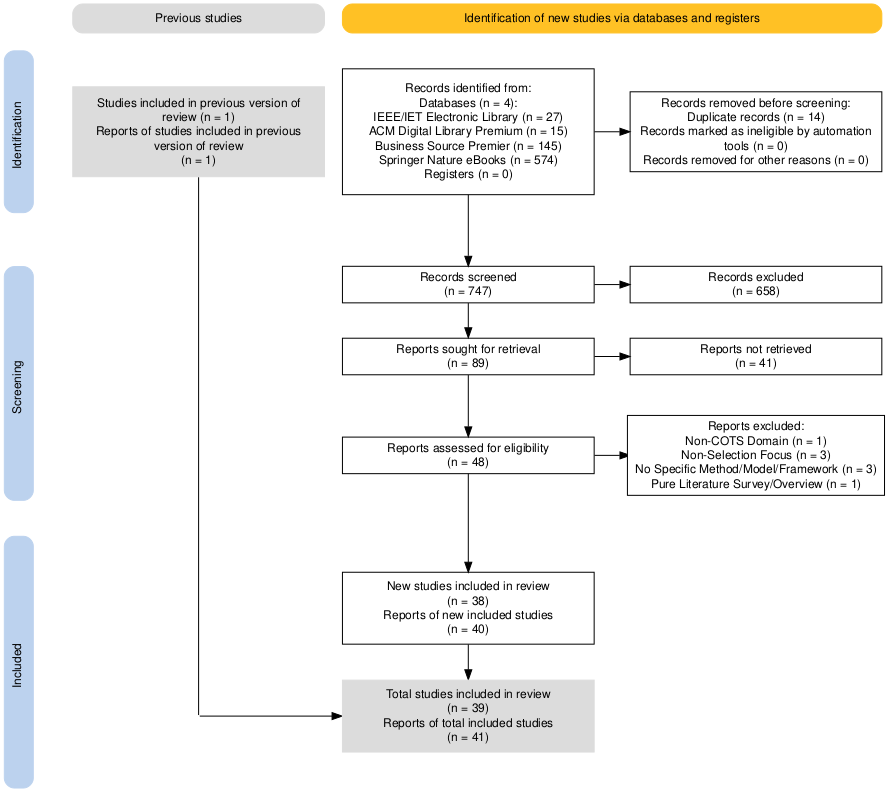
\includegraphics[width=0.85\textwidth]{appendix/prisma_flowchart.png}
\caption{PRISMA 2020 Flussdiagramm des Literaturauswahlprozesses}
\label{fig:prisma_flowchart}
\end{figure}

Die initiale Datenbankabfrage lieferte ein Bruttoergebnis von insgesamt $N = 761$ Datensätzen. Diese verteilten sich wie folgt auf die genutzten Suchräume: SpringerLink steuerte mit $n = 574$ Dokumenten den größten Anteil bei, gefolgt von EBSCOhost mit $n = 145$ Treffern, IEEE Xplore mit $n = 27$ sowie der ACM Digital Library mit $n = 15$ Primärdokumenten. Vor Beginn des inhaltlichen Screenings wurden automatisierte und manuelle Dublettenprüfungen durchgeführt, bei denen $n = 14$ identische Mehrfachtreffer über Datenbankgrenzen hinweg identifiziert und entfernt wurden. Der bereinigte Ausgangsdatenbestand umfasste somit $N = 747$ eindeutige Datensätze.

Der Selektionsprozess vollzog sich anschließend über drei sequenzielle Screening-Stufen (Practical Screens):
\begin{enumerate}
    \item \textbf{Practical Screen 1 (Titel- und Abstract-Screening):} Sämtliche $N = 747$ Datensätze wurden anhand vordefinierter Einschluss- und Ausschlusskriterien auf ihren thematischen Bezug zu COTS-Auswahlmethoden geprüft. In dieser Stufe wurden $n = 599$ Publikationen ausgeschlossen, da sie entweder rein theoretische Abhandlungen ohne konkrete Methodik darstellten, sich ausschließlich auf In-House-Softwareentwicklung bezogen oder keine Entscheidungsmodelle behandelten. Es verblieben $n = 148$ Arbeiten für das nachfolgende Screening.
    \item \textbf{Practical Screen 2 (Relevanz- und Kontextprüfung):} Die verbliebenen $n = 148$ Treffer wurden einer vertieften Prüfung der Zielsetzung unterzogen. Hierbei schieden weitere $n = 59$ Publikationen aus, die lediglich allgemeine IT-Beschaffungsaspekte ohne mathematische oder strukturelle Evaluierungsmodelle behandelten. Dies führte zu einer Zwischensumme von $n = 89$ potenziell relevanten Studien.
    \item \textbf{Volltextabruf und Practical Screen 3 (Volltextprüfung):} Von den $n = 89$ selektierten Studien konnten $n = 48$ Volltexte erfolgreich über universitäre Lizenzen und Open-Access-Repositorien abgerufen werden, während $n = 41$ Arbeiten aufgrund fehlender Subskriptionen oder veralteter Verlagsarchive nicht beschaffbar waren. Die eingehende methodische Volltextprüfung der $n = 48$ zugänglichen Arbeiten führte zum Ausschluss von weiteren $n = 8$ Publikationen, da diese unvollständige Formelapparate aufwiesen oder redundante Teilpublikationen darstellten.
\end{enumerate}

Ergänzend zu den Datenbanktreffern wurde ein zentraler Proposal-Report aus der grauen Literatur beziehungsweise akademischen Qualifikationsarbeiten hinzugefügt ($n = 1$). Somit umfasst das finale Analysekorpus exakt $N = 41$ Berichte, welche sich auf 40 eindeutige Primärstudien verteilen (da die Arbeiten von \cite{MC9UMXZZ} und \cite{9F79VAAB} auf derselben grundlegenden MiHOS-Methodik basieren).

\subsubsection{Demografische und zeitliche Analyse der Literatur}

Die quantitative Auswertung der $N = 41$ finalen Berichte offenbart prägnante Muster hinsichtlich der zeitlichen Verteilung, der Publikationsmedien sowie der methodischen Qualität.

\begin{figure}[htbp]
\centering
\begin{adjustbox}{width=0.9\textwidth}
\begin{tabular}{llcc}
\toprule
\textbf{Zeitraum (Epoche)} & \textbf{Methodischer Schwerpunkt} & \textbf{Anzahl Studien ($N=41$)} & \textbf{Prozentualer Anteil} \\
\midrule
2000--2007 (Epoche 1) & Frühe Heuristiken \& Klassisches MCDM & 14 & 34,1 \% \\
2008--2016 (Epoche 2) & Mathematische Optimierung \& Mismatch-Ära & 15 & 36,6 \% \\
2017--2025 (Epoche 3) & Hybride MCDM-Pipelines \& Soft Computing & 12 & 29,3 \% \\
\bottomrule
\end{tabular}
\end{adjustbox}
\caption{Zeitliche Verteilung der analysierten Primärstudien über die drei Epochen}
\label{tab:epochen_verteilung}
\end{figure}

Wie in Tabelle~\ref{tab:epochen_verteilung} verdeutlicht, verteilt sich das Veröffentlichungsaufkommen bemerkenswert gleichmäßig über das Beobachtungsvierteljahrhundert:
\begin{itemize}
    \item Die erste Phase (2000--2007) umfasst 14 Studien (34,1 \%) und ist geprägt vom Übergang von unsystematischen Checklisten hin zu formalen hierarchischen Gewichtungsmethoden wie dem Analytic Hierarchy Process (AHP) sowie ersten Outranking-Ansätzen.
    \item Die zweite Phase (2008--2016) stellt mit 15 Publikationen (36,6 \%) den quantitativen Höhepunkt dar. Diese Ära zeichnet sich durch die mathematische Formulierung als exakte kombinatorische Optimierungsprobleme (z.\,B. 0-1 Ganzzahlige Lineare Programmierung) sowie die Integration der Fuzzy-Glaubwürdigkeitstheorie aus.
    \item Die dritte Phase (2017--2025) umfasst 12 Berichte (29,3 \%) und reflektiert die Konsolidierung in mehrstufige Hybridsysteme (z.\,B. Delphi-FAHP-PROMETHEE), die Nutzung nicht-parametrischer Effizienzanalysen (DEA) sowie evidenzbasierte Soft-Computing-Ansätze (Dempster-Shafer-Theorie).
\end{itemize}

Hinsichtlich der Veröffentlichungskanäle dominiert der Bereich der internationalen Konferenzbände und renommierten Fachzeitschriften aus dem Software Engineering und Operations Research. Zu den primären Outlets gehören Journal-Publikationen der Verlage IEEE (z.\,B. \textit{IEEE Transactions on Software Engineering}), Elsevier (\textit{Information and Software Technology}, \textit{Expert Systems with Applications}), Springer (\textit{Software Quality Journal}) sowie ACM.

\subsubsection{Bewertung der methodischen Qualität}

Zur Objektivierung der wissenschaftlichen Fundierung wurden alle $N = 41$ Studien einem formalen Qualitätsbewertungsverfahren (\textit{Quality Appraisal}, QA) unterzogen. Das Bewertungsraster umfasst 8 binär beziehungsweise ordinal skalierte Kriterien ($QA_1$ bis $QA_8$), welche unter anderem das Vorhandensein einer klaren Problemdefinition, die mathematische Vollständigkeit des Evaluierungsmodells, das Vorhandensein empirischer Validierungen (Fallstudien oder Experimente), die Transparenz der Kriterienkataloge sowie das Bereitstellen von Software-Tools zur Entscheidungsunterstützung bewerten. Jede Studie konnte somit einen Gesamtwert zwischen 0,0 und 8,0 Punkten erreichen.

Die Einteilung erfolgt in drei Evidenz- und Qualitätsstufen:
\begin{enumerate}
    \item \textbf{High Rigor (Score 6,0 bis 8,0):} Insgesamt $N = 30$ Studien (73,2 \%) erreichten diese höchste Qualitätsstufe. Diese Arbeiten zeichnen sich durch eine lückenlose mathematische Formalisierung, nachvollziehbare Validierungsszenarien und eine detaillierte Diskussion der methodischen Grenzen aus (z.\,B. \cite{LZQJ6M4X, MC9UMXZZ, 8VHUMEKY, NZJEEPAC, LNQHES84}).
    \item \textbf{Medium Rigor (Score 3,0 bis 5,0):} $N = 9$ Studien (22,0 \%) wurden dieser mittleren Kategorie zugeordnet. Diese Arbeiten weisen zwar innovative methodische Ansätze auf, zeigen jedoch Schwächen in der empirischen Validierung oder nutzen vereinfachte Kriterienkataloge ohne domänenspezifische Taxonomie (z.\,B. \cite{CZZ6XQZJ, VUVLUN85, JT5X3FIG}).
    \item \textbf{Low Rigor (Score 0,0 bis 2,0):} Lediglich $N = 2$ Arbeiten (4,9 \%) fielen in den Bereich niedriger Qualität, da es sich um reine Konzeptskizzen ohne mathematischen Beweis oder praktische Erprobung handelte.
\end{enumerate}

Der hohe Anteil von über 73 \% an Studien der höchsten Qualitätsstufe unterstreicht die Eignung des identifizierten Literaturkorpus als verlässliche Datengrundlage für die nachfolgende mathematische und morphologische Synthese.

\subsection{Evolutionäre Abbildung der COTS-Auswahlmethoden}
\label{subsec:evolutionaere_abbildung}

Die induktive Analyse des 25-jährigen Forschungszeitraums gestattet die Rekonstruktion eines dreiphasigen Paradigmenwechsels in der COTS-Softwareevaluierung. Die Entwicklung verläuft von einfachen ad-hoc Gewichtungsschemata hin zu hochkomplexen, mehrstufigen Soft-Computing-Pipelines. Die einzelnen Epochen werden nachfolgend hinsichtlich ihrer theoretischen Paradigmen, mathematischen Verfahren, Wandelstreiber und methodischen Wendepunkte systematisch analysiert.

\subsubsection{Epoche 1 (2000--2007): Frühe Heuristiken und klassisches MCDM}

Die Entstehungsphase der wissenschaftlichen COTS-Auswahlforschung war geprägt von dem Bestreben, rein subjektive, unstrukturierte Checklisten der industriellen Praxis durch formale multikriterielle Entscheidungsmodelle (\textit{Multi-Criteria Decision Making}, MCDM) zu ersetzen. In Unternehmen herrschte bis zur Jahrtausendwende die Praxis vor, Softwareprodukte anhand diffuser Anforderungslisten zu bewerten, was regelmäßig zu Fehleinschätzungen, Kostenüberschreitungen und unvorhergesehenen Schnittstellenproblemen führte.

Frühe Pionierarbeiten führten die Outranking-Methodik in die Softwareauswahl ein. So demonstrierten \cite{LZQJ6M4X} den Einsatz von ELECTRE-TRI, um Kandidatenprodukte auf Basis von Schwellenwerten in geordnete Qualitätskategorien einzusortieren. \cite{M3B2D3GD} erweiterten diesen Ansatz durch die Kombination von ELECTRE II mit der Strukturierung des Qualitätsstandards ISO/IEC 9126, um nicht-homogene Metriken zu aggregieren und die Fallen arithmetischer gewichteter Summen zu vermeiden. Parallel dazu wurde der Analytic Hierarchy Process (AHP) nach Saaty zu einer dominanten Methode für die hierarchische Kriteriengewichtung. \cite{FCYW9EWJ} entwickelten ein mehrstufiges Selektionsmodell, das initiale Screening-Cutoffs mit AHP-Gewichtungen kombiniert, während \cite{DAU8NSK8} AHP gezielt zur Auswahl komplexer CRM-Unternehmenssoftware einsetzten. Um die bei AHP auftretenden paarweisen Vergleichskaskaden bei großen Kriterienkatalogen zu begrenzen, kombinierten \cite{U5JPV4SF} den Analytic Network Process (ANP) mit der TOPSIS-Methode (\textit{Technique for Order of Preference by Similarity to Ideal Solution}), wodurch Wechselwirkungen zwischen Kriterien mathematisch berücksichtigt werden konnten.

Neben rein attributbasierten Bewertungsverfahren entstanden erste zielorientierte Ansätze des Requirements Engineering. \cite{TLB687YL} formulierte ein leichtgewichtiges goal-orientiertes Selektionsframework, das Systemziele direkt mit COTS-Produktfähigkeiten abgleicht. \cite{8XNYS4M9} erweiterten die AGORA-Methodik (\textit{Attributed Goal-Oriented Requirements Analysis}), um Qualitätsattribute in Zielgraph-Strukturen systematisch auszubalancieren und Zielkonflikte quantitativ zu bewerten. In ähnlicher Weise verband das CARE-Framework (\textit{COTS-Based Requirements Engineering}) von \cite{6RNULWVY} den modellgetriebenen Entwurf mit NFR-Zielgraphen (\textit{Non-Functional Requirements}), um die Einhaltung architektonischer Randbedingungen abzusichern. \cite{CZZ6XQZJ} adressierten das Problem verteilter Stakeholder-Interessen durch das NeMo-CoSe-Modell, welches Win-Win-Anforderungsverhandlungen mit spieltheoretischen Gleichgewichtskonzepten und agentenbasierten Verhandlungssystemen verknüpfte. Erste Ansätze zur expliziten Modellierung unsicherer Vendor-Spezifikationen nutzten Bayes'sche Netze zur Berechnung bedingter Wahrscheinlichkeiten der Kriterienerfüllung \cite{QDUNCXFC} sowie unscharfe Mengen (\textit{Fuzzy Sets}) zur Modellierung vager Produktfunktionalitäten \cite{CI86GRRG}.

\textbf{Methodische Wendepunkte der Epoche 1:}
Zwei fundamentale Arbeiten markierten das Ende der ersten Phase und leiteten den Übergang zur Optimierungsära ein:
\begin{enumerate}
    \item \textbf{Interaktive kombinatorische Pareto-Optimierung (Odin):} \cite{ZQMG69VT} brachten mit dem Tool Odin den Nachweis, dass die Vorgabe starrer A-priori-Gewichtungen bei der Auswahl mehrkomponentiger Softwarearchitekturen zu suboptimalen Systemen führt. Sie führten die multikriterielle kombinatorische Optimierung (\textit{Multiobjective Combinatorial Optimization}, MOCO) ein, bei der zunächst der Raum Pareto-effizienter Produktkombinationen berechnet wird, welchen Entscheidungsfinder anschließend interaktiv erkunden können.
    \item \textbf{Formalisierung des Mismatch-Managements (MiHOS):} Die Arbeiten von \cite{MC9UMXZZ} und \cite{9F79VAAB} etablierten das MiHOS-Framework (\textit{Mismatch Handling aware COTS Selection}). Sie zeigten auf, dass COTS-Software selten perfekt zu den Systemanforderungen passt und die Evaluation daher zwingend die nachgelagerten Kosten und Risiken der Fehlerbehebung (\textit{Mismatch Resolution} durch Wrapper, Customizing oder Prozessanpassungen) unter beschränkten Budgets einbeziehen muss.
\end{enumerate}

\subsubsection{Epoche 2 (2008--2016): Mathematische Optimierung und Mismatch-Ära}

Die zweite Epoche war gekennzeichnet durch eine Mathematisierung des Selektionsproblems. An die Stelle isolierter Einzelproduktbewertungen trat die Sichtweise, dass moderne Softwaresysteme aus einer Vielzahl miteinander wechselwirkender COTS-Komponenten, Komponentenarchitekturen und Cloud-Diensten zusammengesetzt werden müssen.

Ein zentraler Schwerpunkt lag auf der Formulierung exakter mathematischer Programmierungsmodelle. \cite{VUVLUN85} entwickelten 0-1 bi-kriterielle ganzzahlige Programmierungsmodelle (\textit{0-1 Integer Linear Programming}, ILP), die unter Einhaltung fester Systembudgets die funktionale Abdeckung maximieren und gleichzeitig die Gesamtkosten minimieren. \cite{MZ8JHDYA} erweiterten den interaktiven MOCO-Ansatz im Atana-Framework, indem sie exakte Enumerationsalgorithmen mit metaheuristischen Suchverfahren (NSGA-II) kombinierten, um auch großdimensionale modulare Komponentensysteme optimieren zu können.

Ein wesentlicher Wandelstreiber dieser Phase war die Erkenntnis, dass Eingabeparameter in der Softwareevaluierung (wie Ausführungszeiten, Zuverlässigkeitswerte oder Anpassungsaufwände) mit hoher epistemischer Unsicherheit behaftet sind. Um dieser Vagheit gerecht zu werden, hielt die mathematische Fuzzy-Optimierung Einzug:
\begin{itemize}
    \item \cite{6YJHIVHG} formulierten ein fuzzy-interaktives multi-objektives 0-1 ganzzahliges nichtlineares Programmierungsmodell, das mithilfe der Zimmermann'schen Fuzzy-Programmierung gelöst wird.
    \item \cite{P9SATBH5} entwickelten ein fuzzy multi-objektives Optimierungsmodell für modulare Systeme, welches Kosten, Ausführungszeiten und Zuverlässigkeit unter unscharfen Nebenbedingungsgrenzen gleichzeitig optimiert.
    \item \cite{JX4RDRDU} sowie \cite{B7ZTQCZZ} führten die credibilistische Glaubwürdigkeitstheorie (\textit{Credibility Theory}) in die COTS-Auswahl ein. Durch die Nutzung von Erwartungswert-Operatoren und chance-constrained Programmierung schufen sie Modelle, die trotz unscharfer Parameter pareto-optimale Kompromisslösungen garantieren.
    \item \cite{VRTXHQI7} kombinierten adaptive AHP-Strukturen mit Genetischen Algorithmen (GA), um Skalierungsinkonsistenzen bei dynamischen Kriterienanpassungen in mehrkomponentigen Systemen zu überwinden.
\end{itemize}

Parallel zur mathematischen Optimierung brachte Epoche 2 operative Entscheidungsunterstützungssysteme (\textit{Decision Support Systems}, DSS) hervor. \cite{8VHUMEKY} präsentierten mit Plato (\textit{Planning Tool}) eine vollständig automatisierte, evidenzbasierte Evaluierungsplattform auf Basis von ISO/IEC 25010 für die langfristige Softwarearchivierung. \cite{U4E7VXQU} entwickelten das hybride wissensbasierte System HKBS, welches regelbasierte IF-THEN-Logiken mit Benutzerpräferenzfiltern vereint. \cite{WZM7DUBY} schuf das COTS-ESF-Framework (\textit{COTS Software Evaluation and Selection Framework}), welches Prozessmodelle, ISO-Standard-Kataloge und Gap-Analysen in dem dedizierten Software-Tool DM-PT zusammenführt.

Ergänzend wurden domänenspezifische Evaluierungsmodelle entwickelt, etwa von \cite{W8P543Y2} für Cloud-SaaS-ERP-Systeme auf Basis von Service-Level-Agreements (SLA), von \cite{LYMHTPXS} für Business Process Management (BPM)-Engines sowie von \cite{JT5X3FIG}, die mit der GRADE-Taxonomie einen empirischen Begriffsrahmen für Build-or-Buy-Entscheidungen etablierten.

\subsubsection{Epoche 3 (2017--2025): Hybrid MCDM, Soft Computing und Evidential Reasoning}

Die aktuelle Epoche zeichnet sich durch die Synergie und Konsolidierung zuvor getrennter Methodenstränge aus. Statt isolierter Einzelverfahren dominieren mehrstufige hybride Decision-Pipelines, welche Gruppenkonsensverfahren, unscharfe Kriteriengewichtungen und fortschrittliche Ranking- beziehungsweise Effizienzanalysen nahtlos miteinander verknüpfen.

Ein charakteristischer Trend ist die Verknüpfung von Fuzzy-AHP mit komplementären Bewertungsverfahren:
\begin{itemize}
    \item \cite{NZJEEPAC} entwarfen eine mehrstufige Architektur, die ein modifiziertes Delphi-Verfahren zur Eliminierung von Experten-Bias, Chang's Fuzzy AHP (FAHP) zur Kriteriengewichtung und PROMETHEE zur Behandlung von Outranking-Beziehungen bei Cloud-Plattformen kombiniert.
    \item \cite{QNWK8SAP} integrierten AHP mit der VIKOR-Methode, um maximale Gruppennützlichkeit bei gleichzeitig minimalem individuellen Bedauern des Entscheiders zu realisieren.
    \item \cite{5BBYQCJB} nutzten dreieckige Fuzzy-Zahlen im FAHP-Kontext, um linguistische Ambiguitäten bei der Auswahl komplexer ERP-Gesamtsysteme präzise abzubilden.
\end{itemize}

Ein weiterer Durchbruch der Epoche 3 liegt in der Etablierung nicht-parametrischer Effizienzanalysen und distanzbasierter Metriken. \cite{YVWGHAWQ} wandten die Data Envelopment Analysis (DEA) in Verbindung mit Fuzzy-Zahlen an, um die relative Effizienz von COTS-Produkten zu messen, ohne dass Entscheider Vorab-Kriteriengewichtungen festlegen müssen. \cite{9BLXY3EP} sowie \cite{FVINCQ89} formulierten den \textit{Fuzzy Modified Distance-Based Approach} (FMDBA). Unter Nutzung 7-stufiger linguistischer Skalen berechnet FMDBA die mathematische Distanz von Softwarealternativen zu idealen und anti-idealen Referenzpunkten direkt auf den Kriterienbäumen des Qualitätsstandards ISO/IEC 25010. \cite{8KF4HAZS} kombinierten TOPSIS-Distanzmaße mit interaktiver fuzzy-multiobjektiver Programmierung.

Einen herausragenden methodischen Fortschritt stellt die Behandlung extremer Nicht-Wissen-Zustände und widersprüchlicher Expertenmeinungen dar. \cite{LNQHES84} wendete die Dempster-Shafer-Evidenztheorie (\textit{Evidential Reasoning}, ER) an. Mithilfe des Software-Tools IDS (\textit{Intelligent Decision System}) gelingt es hierbei, unvollständige Daten und Glaubensmassen (\textit{Belief Mass}) mathematisch korrekt zu aggregieren. Im Bereich industrieller Komponenten wendete \cite{RRU375GB} das Expertenwerkzeug IoT PRISM zur AHP-basierten Plattformauswahl an. Schließlich unterstreicht die systematische Übersicht von \cite{LPC92LAP} den dringenden Bedarf, die verbliebene Lücke zwischen hochkomplexen theoretischen MCDM-Modellen und der industriellen Anwendungspraxis durch benutzerfreundliche DSS-Automatisierung zu schließen.

\subsubsection{Vollständige Epochen-Synthese-Tabelle}

In Tabelle~\ref{tab:epochen_synthese} sind alle $N = 41$ analysierten Berichte der 40 Primärstudien chronologisch erfasst und ihren jeweiligen Entwicklungsphasen nebst Zuordnungsgrund und Wandelstreiber eindeutig zugewiesen.

\begin{longtable}{p{0.12\textwidth} p{0.22\textwidth} p{0.18\textwidth} p{0.22\textwidth} p{0.16\textwidth}}
\caption{Synthese der 41 Primärstudien im 3-Epochen-Evolutionsmodell} \label{tab:epochen_synthese} \\
\toprule
\textbf{Autoren \& Jahr} & \textbf{Zugewiesene Epoche} & \textbf{Zuordnungsgrundlage} & \textbf{Wandelstreiber} \\
\midrule
\endfirsthead
\caption[]{Synthese der 41 Primärstudien im 3-Epochen-Evolutionsmodell (Fortsetzung)} \\
\toprule
\textbf{Autoren \& Jahr} & \textbf{Zugewiesene Epoche} & \textbf{Zuordnungsgrundlage} & \textbf{Wandelstreiber} \\
\midrule
\endhead
\bottomrule
\endfoot
\bottomrule
\endlastfoot

\cite{LZQJ6M4X} & Epoche 1 (2000--2007) & Frühe ELECTRE-TRI Outranking-Kategorisierung & Ablösung subjektiver Checklisten durch Outranking \\
\cite{M3B2D3GD} & Epoche 1 (2000--2007) & ELECTRE II gekoppelt mit ISO 9126 Qualitätsmodell & Vermeidung arithmetischer Summen-Fallen \\
\cite{QDUNCXFC} & Epoche 1 (2000--2007) & Bayes'sche Netze für Kriterienwahrscheinlichkeiten & Probabilistische Risikomodellierung \\
\cite{FCYW9EWJ} & Epoche 1 (2000--2007) & Mehrstufiges Screening mit AHP-Hierarchie & Hierarchische Kriterienstrukturierung \\
\cite{DAU8NSK8} & Epoche 1 (2000--2007) & AHP-Anwendung auf CRM-Softwareauswahl & Strukturierte Unternehmenssoftware-Beschaffung \\
\cite{TLB687YL} & Epoche 1 (2000--2007) & Leichtgewichtiges goal-orientiertes Matching & Brücke zwischen Requirements und COTS \\
\cite{CI86GRRG} & Epoche 1 (2000--2007) & Fuzzy Sets für komponentenbasierte Spezifikationen & Behandlung vager Herstellerspezifikationen \\
\cite{CZZ6XQZJ} & Epoche 1 (2000--2007) & NeMo-CoSe: Anforderungsverhandlung \& Spieltheorie & Konfliktlösung bei Stakeholder-Anforderungen \\
\cite{U5JPV4SF} & Epoche 1 (2000--2007) & 5-Phasen-Modell aus ANP und modifiziertem TOPSIS & Abbildung von Kriterien-Wechselwirkungen \\
\cite{8XNYS4M9} & Epoche 1 (2000--2007) & AGORA-Zielgrapherweiterung für Konfliktanalysen & Quantifizierung von Zielkonflikten \\
\cite{6RNULWVY} & Epoche 1 (2000--2007) & CARE Framework: NFR-Zielgraphen \& MDE & Architektureinhaltung durch NFR-Rückverfolgung \\
\cite{MC9UMXZZ} & Epoche 1 (2000--2007) & MiHOS: Mismatch-Klassifikation \& ILP-Solver & Bewusstsein für post-evaluative Anpassungskosten \\
\cite{9F79VAAB} & Epoche 1 (2000--2007) & MiHOS Dissertation: 6 Mismatch-Typen \& MiHOS-PT & Formale Mismatch-Behebung unter Budgetgrenzen \\
\cite{ZQMG69VT} & Epoche 1 (2000--2007) & Odin Tool: MOCO \& interaktive Pareto-Erkundung & Vermeidung starrer A-priori-Kriteriengewichte \\
\cite{MZ8JHDYA} & Epoche 2 (2008--2016) & Atana: MOCO mit NSGA-II Metaheuristik & Skalierung auf mehrkomponentige Systeme \\
\cite{WBGP3ETU} & Epoche 2 (2008--2016) & Multipfad-Prozessmodell \& Perzentil-Matching & Standardisierung von COTS-Integrationsabläufen \\
\cite{8VHUMEKY} & Epoche 2 (2008--2016) & Plato DSS-Plattform für evidenzbasierte Auswahl & Automatisierte langfristige Software-Preservation \\
\cite{VUVLUN85} & Epoche 2 (2008--2016) & 0-1 bi-kriterielle ganzzahlige Programmierungsmodelle & Exakte mathematische Budget-Optimierung \\
\cite{U4E7VXQU} & Epoche 2 (2008--2016) & HKBS: Experten-Regelsystem mit IF-THEN Logik & Automatisierte Wissensverarbeitung in DSS \\
\cite{6YJHIVHG} & Epoche 2 (2008--2016) & Fuzzy interaktives 0-1 MINLP Modell & Modellierung unscharfer Systemparameter \\
\cite{VRTXHQI7} & Epoche 2 (2008--2016) & Adaptives AHP gekoppelt mit Genetischen Algorithmen & Beherrschung dynamischer Kriterienänderungen \\
\cite{W8P543Y2} & Epoche 2 (2008--2016) & QoS-basiertes MCDM-Modell für SaaS-ERP & Anpassung an Cloud-SLAs und Service-Qualität \\
\cite{WZM7DUBY} & Epoche 2 (2008--2016) & COTS-ESF Framework \& DM-PT Software-Tool & Operatives Gesamtmodell mit ISO 9126 Bezug \\
\cite{LYMHTPXS} & Epoche 2 (2008--2016) & Strukturierte Evaluierungsmethode für BPM-Engines & Domänenspezifische Middleware-Evaluierung \\
\cite{JX4RDRDU} & Mehlawat \& Gupta (2015a) & Epoche 2 (2008--2016) & Credibilistisches multi-objektives ILP Modell & Mathematische Glaubwürdigkeitstheorie \\
\cite{P9SATBH5} & Kaur et al. (2015) & Epoche 2 (2008--2016) & Fuzzy multi-objektive modulare Optimierung & Zeit-Kosten-Zuverlässigkeits-Optimierung \\
\cite{B7ZTQCZZ} & Mehlawat \& Gupta (2015b) & Epoche 2 (2008--2016) & Hybrid TOPSIS mit credibilistischem Chance-Constraint & Kompensatorische Pareto-Optimalität \\
\cite{JT5X3FIG} & Wohlin et al. (2016) & Epoche 2 (2008--2016) & GRADE-Taxonomie für Komponentenauswahl & Empirische Begriffsordnung für Build/Buy \\
\cite{DFASRUVC} & Khatri et al. (2016) & Epoche 2 (2008--2016) & Generisches AHP- und score-basiertes Framework & Standardisierung von AHP-Beschaffungsabläufen \\
\cite{QNWK8SAP} & Anon. (2017) & Epoche 3 (2017--2025) & Hybride AHP-VIKOR Evaluierungsmethodik & Kompromiss-Ranking bei Zielkonflikten \\
\cite{NZJEEPAC} & Hanine et al. (2017) & Epoche 3 (2017--2025) & Delphi-Fuzzy AHP-PROMETHEE Hybrid-Pipeline & Bias-freier Gruppenkonsens mit Outranking \\
\cite{UK2X9C4W} & Chatzipetrou et al. (2020) & Epoche 3 (2017--2025) & Cumulative Voting (\$100 Test) für Priorisierung & Empirische Validierung von Priorisierungen \\
\cite{5BBYQCJB} & Bhatt et al. (2021) & Epoche 3 (2017--2025) & Fuzzy AHP mit dreieckigen Fuzzy-Zahlen für ERP & Bewältigung linguistischer Subjektivität \\
\cite{RRU375GB} & Lempert (2021) & Epoche 3 (2017--2025) & AHP-Auswahl mit Screening \& IoT PRISM Tool & Werkzeugunterstützung im IoT-Umfeld \\
\cite{UFCEV52H} & Kalantari et al. (2021) & Epoche 3 (2017--2025) & Fuzzy multiobjektive nichtlineare Optimierung & Dynamic Requirements \& Interaktionsgrenzen \\
\cite{9BLXY3EP} & Anon. (2022) & Epoche 3 (2017--2025) & Fuzzy Modified Distance-Based Approach (FMDBA) & Distanzmetriken auf ISO 25010 Qualitätsbäumen \\
\cite{FVINCQ89} & Garg (2022) & Epoche 3 (2017--2025) & FMDBA mit 7-stufiger linguistischer Skala & Präzisierung distanzbasierter Rankings \\
\cite{8KF4HAZS} & Verma et al. (2022) & Epoche 3 (2017--2025) & TOPSIS mit interaktiver Fuzzy-Programmierung & Synthese aus Distanzmaß und Optimierung \\
\cite{YVWGHAWQ} & Gupta et al. (2022) & Epoche 3 (2017--2025) & Data Envelopment Analysis (DEA) mit Fuzzy-Zahlen & Nicht-parametrische Effizienzmessung \\
\cite{LNQHES84} & Nabot (2025) & Epoche 3 (2017--2025) & Dempster-Shafer Evidential Reasoning \& IDS Tool & Evidenzbasierte Glaubensmassen aggregieren \\
\cite{LPC92LAP} & Taherdoost \& Mohebi (2025) & Epoche 3 (2017--2025) & Systematische Übersicht über 41 MCDM-Techniken & Brückenschlag zwischen Theorie und Praxis \\
\end{longtable}

\subsection{Morphologische Analyse der COTS-Auswahlmethoden}
\label{subsec:morphologische_analyse}

Um die strukturelle Beschaffenheit, die Variationsbreite und die methodischen Lücken der existierenden COTS-Auswahlverfahren frei von Beschränkungen rein quantitativer Taxonomien zu untersuchen, wird die von Fritz Zwicky begründete \textit{General Morphological Analysis} (GMA) angewendet \cite{Z6N6V5L9}. Gemäß Ritchey stellt die GMA eine systematische Methode dar, um mehrdimensionale, nicht-quantifizierbare Problemkomplexe zu strukturieren, indem der Gesamtraum möglicher Lösungsarchitekturen in diskrete Parameter und gegenseitig ausschließende Wertzustände zerlegt wird.

\subsubsection{Das Morphologische Feld}

Auf Basis der Synthese des Literaturkorpus wurde ein 6-dimensionales orthgonales morphologisches Feld konstruiert ($n = 6$). Die Parameter $P_1$ bis $P_6$ sowie ihre Wertzustände $v_{i,j}$ repräsentieren die Kerndimensionen der methodischen Gestaltung von COTS-Auswahlverfahren:

\begin{enumerate}
    \item \textbf{$P_1$: Mathematisches Entscheidungsmodell (Mathematical Decision Model Family):}
    \begin{itemize}
        \item $v_{1.1}$ -- \textit{Outranking \& Paarweise MCDM}: Distanz- oder Präferenz-Rankings basierend auf paarweisen Vergleichen (AHP, ANP, TOPSIS, ELECTRE, VIKOR, PROMETHEE, FMDBA). [$N = 18$ Studien]
        \item $v_{1.2}$ -- \textit{Mathematische Programmierung \& Optimierung}: Exakte oder heuristische beschränkte Optimierungsmodelle (MOCO, ILP, 0-1 Ganzzahlige Programmierung, MINLP, DEA). [$N = 12$ Studien]
        \item $v_{1.3}$ -- \textit{Fuzzy \& Evidenzbasierte Soft Computing-Strukturen}: Soft-Computing-Architekturen mit Fokus auf Unsicherheitsgrenzen oder Evidenzaggregation (Fuzzy Sets, Dempster-Shafer ER, Bayes'sche Netze). [$N = 3$ Studien]
        \item $v_{1.4}$ -- \textit{Qualitative \& Deskriptive Heuristiken}: Regelbasierte Systeme, Zielgraph-Matching, Priorisierungs-Voting oder deskriptive Prozesstaxonomien (Rule-Based RBR, Cumulative Voting, Goal Graphs, GRADE). [$N = 8$ Studien]
    \end{itemize}

    \item \textbf{$P_2$: Mismatch-Behandlungsphase (Mismatch Handling Phase):}
    \begin{itemize}
        \item $v_{2.1}$ -- \textit{Pre-Evaluation Screening Cutoff}: Härte-Filter zur Eliminierung nicht-konformer Kandidaten vor der Hauptbewertung. [$N = 7$ Studien]
        \item $v_{2.2}$ -- \textit{In-Evaluation Interactive Trade-Off}: Interaktive Lockockerung von Kriteriengrenzen, Kompromissverhandlungen oder Pareto-Erkundungen während der Evaluation. [$N = 15$ Studien]
        \item $v_{2.3}$ -- \textit{Explicit Post-Evaluation Optimization}: Formale Mismatch-Taxonomien, mathematische Optimierung von Anpassungsmaßnahmen (Customizing/Wrapper) nach dem Ranking. [$N = 3$ Studien]
        \item $v_{2.4}$ -- \textit{Keine / Nicht explizit adressiert}: Behandlung von COTS-Eigenschaften als statische Bewertungsmetriken ohne Mismatch-Kompensation. [$N = 16$ Studien]
    \end{itemize}

    \item \textbf{$P_3$: Kriterien-Standardisierung (Criteria Catalog Standardization):}
    \begin{itemize}
        \item $v_{3.1}$ -- \textit{Standard-basierte Taxonomie}: Kriterienstrukturen, die direkt aus internationalen Normen abgeleitet sind (ISO/IEC 9126, ISO/IEC 25010, IEEE 1061, GRADE). [$N = 8$ Studien]
        \item $v_{3.2}$ -- \textit{Spezifisch-Hierarchisch / Zielgraph}: Projektspezifisch strukturierte Zielbäume oder GQM-Hierarchien (\textit{Goal-Question-Metric}). [$N = 23$ Studien]
        \item $v_{3.3}$ -- \textit{Generisch-Flach / Unstrukturiert}: Ad-hoc-Listen mathematischer Variablen ohne Kriterienhierarchie oder Domänenontologie. [$N = 10$ Studien]
    \end{itemize}

    \item \textbf{$P_4$: Unsicherheits-Behandlung (Uncertainty Handling Mechanism):}
    \begin{itemize}
        \item $v_{4.1}$ -- \textit{Deterministisch / Exakte Werte}: Annahme präziser numerischer Eingabewerte ohne Unsicherheitsmodellierung. [$N = 21$ Studien]
        \item $v_{4.2}$ -- \textit{Possibilistisch / Fuzzy-Logik}: Unscharfe Zugehörigkeitsfunktionen (dreieckige/trapezförmige Fuzzy-Zahlen, FAHP, Type-2 Fuzzy). [$N = 12$ Studien]
        \item $v_{4.3}$ -- \textit{Probabilistisch \& Evidenzbasiert}: Bayes'sche Wahrscheinlichkeiten, Dempster-Shafer Evidenzmassen, Credibility-Theorie. [$N = 8$ Studien]
    \end{itemize}

    \item \textbf{$P_5$: Entscheidungsunterstützungs-Automatisierung (DSS Automation Level):}
    \begin{itemize}
        \item $v_{5.1}$ -- \textit{Vollautomatisierte dedizierte DSS-Software}: Implementierter eigenständiger Prototyp mit Benutzeroberfläche (z.\,B. Odin, MiHOS-PT, Plato, HKBS, DM-PT, IoT PRISM, IDS). [$N = 10$ Studien]
        \item $v_{5.2}$ -- \textit{Solver-gestützte Skriptumgebung}: Nutzung mathematischer Solver (LINGO, MATLAB, R) ohne eigene Benutzeroberfläche. [$N = 9$ Studien]
        \item $v_{5.3}$ -- \textit{Manuell / Konzeptuelles Framework}: Papierbasierte Berechnungen, Formeln oder rein theoretische Leitfäden. [$N = 22$ Studien]
    \end{itemize}

    \item \textbf{$P_6$: Abgedeckter Kriterienumfang (Covered Criteria Scope):}
    \begin{itemize}
        \item $v_{6.1}$ -- \textit{Fokus auf Qualität \& Technik}: Ausschließlich Software-Qualitätsattribute, Performanz und Architektur. [$N = 5$ Studien]
        \item $v_{6.2}$ -- \textit{Fokus auf Business \& Kosten}: Ausschließlich Anbieterstabilität, Lizenzkosten und kaufmännische Eignung. [$N = 0$ Studien]
        \item $v_{6.3}$ -- \textit{Umfassend Multidimensional}: Kombiniert technische, funktionale, kaufmännische und herstellerbezogene Kriterien. [$N = 36$ Studien]
    \end{itemize}
\end{enumerate}

Der theoretische Gesamtraum $N$ aller möglichen Methodenprofil-Konfigurationen berechnet sich aus dem Produkt der Wertzustände der orthogonalen Parameter:
\begin{equation}
N = \prod_{i=1}^{6} |v_i| = |v_1| \times |v_2| \times |v_3| \times |v_4| \times |v_5| \times |v_6| = 4 \times 4 \times 3 \times 3 \times 3 \times 3 = 1.296
\end{equation}
Es existieren somit theoretisch 1.296 denkbare Methodenkombinationen im morphologischen Feld.

\subsubsection{Ergebnisse der Cross-Consistency Assessment und Inkompatibilitätsregeln}

Nach Ritchey dient das *Cross-Consistency Assessment* (CCA) dazu, den theoretischen Gesamtraum durch die Identifikation logischer, methodischer und empirischer Inkompatibilitäten zwischen Paar-Kombinationen von Parameterzuständen auf den reduzierten Raum konsistenter Konfigurationen einzuschränken. Die formalisierten Unvereinbarkeitsregeln stellen sich wie folgt dar:

\begin{enumerate}
    \item \textbf{Regel 1: Mathematische Optimierung vs. Manuelle Ausführung}
    \begin{equation}
    \text{Condition: } (P_1 = v_{1.2}) \land (P_5 = v_{5.3}) \implies \text{Inkompatibel (Logischer Widerspruch)}
    \end{equation}
    \textit{Begründung:} Multikriterielle ganzzahlige Programmierungen (0-1 ILP, MINLP) und kombinatorische Optimierungen (MOCO) sind aufgrund ihrer NP-harten Komplexität manuell auf dem Papier nicht berechenbar. Sie erfordern zwingend den Einsatz von Solver-Engines ($v_{5.2}$) oder DSS-Software ($v_{5.1}$).
    
    \item \textbf{Regel 2: Deterministische Modellierung vs. Unscharfe/Probabilistische Verarbeitungslogik}
    \begin{equation}
    \text{Condition: } (P_4 = v_{4.1}) \land (P_4 \in \{v_{4.2}, v_{4.3}\}) \implies \text{Logisch Ausgeschlossen}
    \end{equation}
    \textit{Begründung:} Ein Entscheidungsmodell kann nicht gleichzeitig exakte deterministische Punktwerte annehmen und beanspruchen, epistemische Vagheit ohne Zugehörigkeitsfunktionen oder Glaubensmassen abzubilden.
    
    \item \textbf{Regel 3: Post-Evaluative Mismatch-Optimierung vs. Rein technischer Kriterienumfang}
    \begin{equation}
    \text{Condition: } (P_2 = v_{2.3}) \land (P_6 = v_{6.1}) \implies \text{Empirisch Inkonsistent}
    \end{equation}
    \textit{Begründung:} Die mathematische Optimierung von Mismatch-Behebungsmaßnahmen (z.\,B. MiHOS) setzt zwingend voraus, dass Anpassungsaufwände gegen kaufmännische Budgets und Anbietersupport abgewogen werden. Eine isolierte Betrachtung rein technischer Metriken entzieht der post-evaluativen Optimierung die ökonomische Entscheidungsgrundlage.
    
    \item \textbf{Regel 4: Vollautomatisierte DSS-Software vs. Unstrukturierte Kriterienlisten}
    \begin{equation}
    \text{Condition: } (P_5 = v_{5.1}) \land (P_3 = v_{3.3}) \implies \text{Empirisch Leerer Raum}
    \end{equation}
    \textit{Begründung:} Eigenständige DSS-Softwareprototypen (wie Plato, Odin, DM-PT oder IDS) benötigen strukturierte Zielgraphen oder ISO-Taxonomien als Eingabe-Ontologie, um Algorithmen automatisiert auszuführen. Unstrukturierte Ad-hoc-Variablenlisten lassen sich nicht in automatisierte Software-Werkzeuge parsen.
\end{enumerate}

\subsubsection{Synthese der 6 Archetypen-Cluster}

Durch die Aggregation der konsistenten Profil-Tupel $[P_1, P_2, P_3, P_4, P_5, P_6]$ lassen sich die 41 Primärstudien in 6 methodische Archetypen-Cluster einteilen:

\begin{itemize}
    \item \textbf{Archetyp A: Klassische MCDM- und Outranking-Systeme}
    \begin{itemize}
        \item \textit{Profilmuster}: $[P_1=v_{1.1}, P_2 \in \{v_{2.1}, v_{2.4}\}, P_3 \in \{v_{3.1}, v_{3.2}\}, P_4=v_{4.1}, P_5 \in \{v_{5.1}, v_{5.3}\}, P_6=v_{6.3}]$
        \item \textit{Repräsentative Studien}: Shyur \cite{U5JPV4SF}, Sarkis \& Sundarraj \cite{FCYW9EWJ}, Colombo \& Francalanci \cite{DAU8NSK8}, Al-Tarawneh (DM-PT) \cite{WZM7DUBY}.
        \item \textit{Durchschnittlicher QA-Score}: 7,2 / 8,0 (Hohe Riggor).
        \item \textit{Charakteristik}: Zerlegt Kriterien in hierarchische Bäume mittels AHP/ANP/TOPSIS. Sehr hohe praktische Intuition, jedoch anfällig für paarweise Vergleichsexplosionen und Rangumkehrungen (\textit{Rank Reversal}).
    \end{itemize}

    \item \textbf{Archetyp B: Kombinatorische Optimierung \& Ressourcen-Allokation}
    \begin{itemize}
        \item \textit{Profilmuster}: $[P_1=v_{1.2}, P_2=v_{2.2}, P_3=v_{3.2}, P_4=v_{4.1}, P_5 \in \{v_{5.1}, v_{5.2}\}, P_6=v_{6.3}]$
        \item \textit{Repräsentative Studien}: Neubauer \& Stummer (Odin) \cite{ZQMG69VT}, Neubauer et al. (Atana) \cite{MZ8JHDYA}, Jha et al. \cite{VUVLUN85}.
        \item \textit{Durchschnittlicher QA-Score}: 6,3 / 8,0.
        \item \textit{Charakteristik}: Formuliert die COTS-Auswahl als MOCO oder 0-1 ILP. Garantiert Pareto-Effizienz ohne subjektive A-priori-Gewichte, erfordert jedoch hohen Rechenaufwand.
    \end{itemize}

    \item \textbf{Archetyp C: Zielorientierte Mismatch-Architekturen}
    \begin{itemize}
        \item \textit{Profilmuster}: $[P_1 \in \{v_{1.2}, v_{1.4}\}, P_2=v_{2.3}, P_3=v_{3.2}, P_4=v_{4.3}, P_5=v_{5.1}, P_6=v_{6.3}]$
        \item \textit{Repräsentative Studien}: Mohamed \& Ruhe (MiHOS) \cite{MC9UMXZZ, 9F79VAAB}, Wanyama \& Far (NeMo-CoSe) \cite{CZZ6XQZJ}, Cechich et al. (AGORA) \cite{8XNYS4M9}, Chung et al. (CARE) \cite{6RNULWVY}.
        \item \textit{Durchschnittlicher QA-Score}: 6,8 / 8,0.
        \item \textit{Charakteristik}: Fokussiert auf die Identifikation von Ziel-Fähigkeiten-Abweichungen und optimiert post-evaluative Anpassungsmaßnahmen über Solver und Verhandlungsmodelle.
    \end{itemize}

    \item \textbf{Archetyp D: Fuzzy-Mathematische Programmierung \& Glaubwürdigkeitsmodelle}
    \begin{itemize}
        \item \textit{Profilmuster}: $[P_1=v_{1.2}, P_2=v_{2.2}, P_3=v_{3.3}, P_4 \in \{v_{4.2}, v_{4.3}\}, P_5=v_{5.2}, P_6=v_{6.3}]$
        \item \textit{Repräsentative Studien}: Mehlawat \& Gupta \cite{B7ZTQCZZ, JX4RDRDU}, Gupta et al. \cite{6YJHIVHG}, Kaur et al. \cite{P9SATBH5}, Kalantari et al. \cite{UFCEV52H}, Verma et al. \cite{8KF4HAZS}.
        \item \textit{Durchschnittlicher QA-Score}: 6,7 / 8,0.
        \item \textit{Charakteristik}: Nutzt Credibility-Theorie und Zimmermann-Fuzzy-Programmierung zur Optimierung unter Parameter-Vagheit. Hohe mathematische Riggor, aber starr auf unstrukturierte Variablenlisten ($v_{3.3}$) fixiert.
    \end{itemize}

    \item \textbf{Archetyp E: Erweiterte hybride Soft-Computing-Systeme}
    \begin{itemize}
        \item \textit{Profilmuster}: $[P_1 \in \{v_{1.1}, v_{1.3}\}, P_2=v_{2.4}, P_3 \in \{v_{3.1}, v_{3.2}\}, P_4 \in \{v_{4.2}, v_{4.3}\}, P_5 \in \{v_{5.1}, v_{5.3}\}, P_6=v_{6.3}]$
        \item \textit{Repräsentative Studien}: Hanine et al. \cite{NZJEEPAC}, Nabot (IDS Tool) \cite{LNQHES84}, Garg (FMDBA) \cite{FVINCQ89, 9BLXY3EP}, Gupta et al. (DEA-Fuzzy) \cite{YVWGHAWQ}, Bhatt et al. \cite{5BBYQCJB}, Anon. (AHP-VIKOR) \cite{QNWK8SAP}.
        \item \textit{Durchschnittlicher QA-Score}: 7,1 / 8,0.
        \item \textit{Charakteristik}: Kombiniert Delphi, FAHP, PROMETHEE, DEA und Evidential Reasoning zur Beherrschung komplexer Bewertungsdaten und unvollständiger Informationen.
    \end{itemize}

    \item \textbf{Archetyp F: Wissensbasierte DSS-Plattformen}
    \begin{itemize}
        \item \textit{Profilmuster}: $[P_1 \in \{v_{1.1}, v_{1.4}\}, P_2 \in \{v_{2.1}, v_{2.2}\}, P_3 \in \{v_{3.1}, v_{3.2}\}, P_4 \in \{v_{4.1}, v_{4.2}\}, P_5=v_{5.1}, P_6=v_{6.3}]$
        \item \textit{Repräsentative Studien}: Becker \& Rauber (Plato) \cite{8VHUMEKY}, Jadhav \& Sonar (HKBS) \cite{U4E7VXQU}, Lempert (IoT PRISM) \cite{RRU375GB}, Wohlin et al. (GRADE) \cite{JT5X3FIG}.
        \item \textit{Durchschnittlicher QA-Score}: 6,7 / 8,0.
        \item \textit{Charakteristik}: Implementiert regelbasierte Expertensysteme oder automatisierte ISO 25010 Evaluierungsplattformen mit hohem Software-Automatisierungsgrad.
    \end{itemize}
\end{itemize}

\subsubsection{Vollständige Morphologische Profil-Tabelle}

In Tabelle~\ref{tab:morphologische_profile} sind die individuellen Profil-Tupel, die Zuordnung zu den 6 Archetypen-Clustern sowie der finale Quality-Appraisal-Score für alle $N = 41$ Arbeiten zusammengestellt.

\begin{longtable}{p{0.10\textwidth} p{0.18\textwidth} p{0.28\textwidth} p{0.24\textwidth} p{0.08\textwidth}}
\caption{Morphologische Profile und Archetypen-Zuordnung aller 41 Studien} \label{tab:morphologische_profile} \\
\toprule
\textbf{Key \& Zitat} & \textbf{Autoren \& Jahr} & \textbf{Morphologisches Profil-Tupel} & \textbf{Archetypen-Cluster} & \textbf{QA-Score} \\
\midrule
\endfirsthead
\caption[]{Morphologische Profile und Archetypen-Zuordnung aller 41 Studien (Fortsetzung)} \\
\toprule
\textbf{Key \& Zitat} & \textbf{Autoren \& Jahr} & \textbf{Morphologisches Profil-Tupel} & \textbf{Archetypen-Cluster} & \textbf{QA-Score} \\
\midrule
\endhead
\bottomrule
\endfoot
\bottomrule
\endlastfoot

\cite{LZQJ6M4X} & Paschetta \& Tsoukiàs (2000) & $[v_{1.1}, v_{2.4}, v_{3.1}, v_{4.1}, v_{5.3}, v_{6.1}]$ & Archetyp A (Klassisches MCDM) & 8/8 \\
\cite{M3B2D3GD} & Blin \& Tsoukiàs (2001) & $[v_{1.1}, v_{2.2}, v_{3.1}, v_{4.1}, v_{5.3}, v_{6.1}]$ & Archetyp A (Klassisches MCDM) & 7/8 \\
\cite{QDUNCXFC} & Morris \& Beling (2001) & $[v_{1.3}, v_{2.4}, v_{3.2}, v_{4.3}, v_{5.3}, v_{6.3}]$ & Archetyp E (Hybrides Soft Comp.) & 8/8 \\
\cite{FCYW9EWJ} & Sarkis \& Sundarraj (2003) & $[v_{1.1}, v_{2.1}, v_{3.2}, v_{4.1}, v_{5.3}, v_{6.3}]$ & Archetyp A (Klassisches MCDM) & 7/8 \\
\cite{DAU8NSK8} & Colombo \& Francalanci (2004) & $[v_{1.1}, v_{2.4}, v_{3.2}, v_{4.1}, v_{5.3}, v_{6.3}]$ & Archetyp A (Klassisches MCDM) & 8/8 \\
\cite{TLB687YL} & Franch (2005) & $[v_{1.4}, v_{2.2}, v_{3.2}, v_{4.1}, v_{5.3}, v_{6.3}]$ & Archetyp C (Goal-Oriented) & 7/8 \\
\cite{CI86GRRG} & Cooper et al. (2005) & $[v_{1.3}, v_{2.4}, v_{3.2}, v_{4.2}, v_{5.3}, v_{6.1}]$ & Archetyp E (Hybrides Soft Comp.) & 7/8 \\
\cite{CZZ6XQZJ} & Wanyama \& Far (2005) & $[v_{1.4}, v_{2.3}, v_{3.2}, v_{4.3}, v_{5.1}, v_{6.3}]$ & Archetyp C (Goal-Oriented) & 3/8 \\
\cite{U5JPV4SF} & Shyur (2006) & $[v_{1.1}, v_{2.1}, v_{3.2}, v_{4.1}, v_{5.3}, v_{6.3}]$ & Archetyp A (Klassisches MCDM) & 8/8 \\
\cite{8XNYS4M9} & Cechich \& Piattini (2006) & $[v_{1.4}, v_{2.2}, v_{3.2}, v_{4.1}, v_{5.3}, v_{6.1}]$ & Archetyp C (Goal-Oriented) & 6/8 \\
\cite{6RNULWVY} & Chung et al. (2006) & $[v_{1.1}, v_{2.2}, v_{3.2}, v_{4.1}, v_{5.3}, v_{6.3}]$ & Archetyp C (Goal-Oriented) & 7/8 \\
\cite{MC9UMXZZ} & Mohamed et al. (2007) & $[v_{1.2}, v_{2.3}, v_{3.2}, v_{4.3}, v_{5.1}, v_{6.3}]$ & Archetyp C (Goal-Oriented) & 8/8 \\
\cite{9F79VAAB} & Mohamed (2007) & $[v_{1.2}, v_{2.3}, v_{3.2}, v_{4.3}, v_{5.1}, v_{6.3}]$ & Archetyp C (Goal-Oriented) & 8/8 \\
\cite{ZQMG69VT} & Neubauer \& Stummer (2007) & $[v_{1.2}, v_{2.2}, v_{3.2}, v_{4.1}, v_{5.1}, v_{6.3}]$ & Archetyp B (Kombin. Optimierung) & 6/8 \\
\cite{MZ8JHDYA} & Neubauer et al. (2008) & $[v_{1.2}, v_{2.2}, v_{3.2}, v_{4.1}, v_{5.1}, v_{6.3}]$ & Archetyp B (Kombin. Optimierung) & 7/8 \\
\cite{WBGP3ETU} & Skroch (2010) & $[v_{1.4}, v_{2.1}, v_{3.2}, v_{4.3}, v_{5.3}, v_{6.3}]$ & Archetyp A (Klassisches MCDM) & 7/8 \\
\cite{8VHUMEKY} & Becker \& Rauber (2010) & $[v_{1.1}, v_{2.2}, v_{3.1}, v_{4.1}, v_{5.1}, v_{6.3}]$ & Archetyp F (Wissensbasierte DSS) & 8/8 \\
\cite{VUVLUN85} & Jha et al. (2010) & $[v_{1.2}, v_{2.2}, v_{3.3}, v_{4.1}, v_{5.2}, v_{6.3}]$ & Archetyp B (Kombin. Optimierung) & 5/8 \\
\cite{U4E7VXQU} & Jadhav \& Sonar (2011) & $[v_{1.4}, v_{2.1}, v_{3.2}, v_{4.2}, v_{5.1}, v_{6.3}]$ & Archetyp F (Wissensbasierte DSS) & 8/8 \\
\cite{6YJHIVHG} & Gupta et al. (2012) & $[v_{1.2}, v_{2.2}, v_{3.3}, v_{4.2}, v_{5.2}, v_{6.3}]$ & Archetyp D (Fuzzy-Math. Progr.) & 7/8 \\
\cite{VRTXHQI7} & Roshanaei et al. (2013) & $[v_{1.1}, v_{2.4}, v_{3.2}, v_{4.2}, v_{5.2}, v_{6.3}]$ & Archetyp D (Fuzzy-Math. Progr.) & 8/8 \\
\cite{W8P543Y2} & Park \& Jeong (2013) & $[v_{1.1}, v_{2.4}, v_{3.2}, v_{4.1}, v_{5.3}, v_{6.3}]$ & Archetyp A (Klassisches MCDM) & 7/8 \\
\cite{WZM7DUBY} & Al-Tarawneh (2014) & $[v_{1.1}, v_{2.1}, v_{3.1}, v_{4.1}, v_{5.1}, v_{6.3}]$ & Archetyp A (Klassisches MCDM) & 8/8 \\
\cite{LYMHTPXS} & Delgado et al. (2015) & $[v_{1.1}, v_{2.4}, v_{3.2}, v_{4.1}, v_{5.3}, v_{6.3}]$ & Archetyp A (Klassisches MCDM) & 6/8 \\
\cite{JX4RDRDU} & Mehlawat \& Gupta (2015a) & $[v_{1.2}, v_{2.2}, v_{3.3}, v_{4.3}, v_{5.2}, v_{6.3}]$ & Archetyp D (Fuzzy-Math. Progr.) & 6/8 \\
\cite{P9SATBH5} & Kaur et al. (2015) & $[v_{1.2}, v_{2.2}, v_{3.3}, v_{4.2}, v_{5.2}, v_{6.3}]$ & Archetyp D (Fuzzy-Math. Progr.) & 7/8 \\
\cite{B7ZTQCZZ} & Mehlawat \& Gupta (2015b) & $[v_{1.2}, v_{2.2}, v_{3.3}, v_{4.3}, v_{5.2}, v_{6.3}]$ & Archetyp D (Fuzzy-Math. Progr.) & 7/8 \\
\cite{JT5X3FIG} & Wohlin et al. (2016) & $[v_{1.4}, v_{2.1}, v_{3.1}, v_{4.1}, v_{5.3}, v_{6.3}]$ & Archetyp F (Wissensbasierte DSS) & 4/8 \\
\cite{DFASRUVC} & Khatri et al. (2016) & $[v_{1.1}, v_{2.4}, v_{3.2}, v_{4.1}, v_{5.3}, v_{6.3}]$ & Archetyp A (Klassisches MCDM) & 5/8 \\
\cite{QNWK8SAP} & Anon. (2017) & $[v_{1.1}, v_{2.4}, v_{3.2}, v_{4.1}, v_{5.3}, v_{6.1}]$ & Archetyp E (Hybrides Soft Comp.) & 7/8 \\
\cite{NZJEEPAC} & Hanine et al. (2017) & $[v_{1.1}, v_{2.4}, v_{3.2}, v_{4.2}, v_{5.3}, v_{6.3}]$ & Archetyp E (Hybrides Soft Comp.) & 7/8 \\
\cite{UK2X9C4W} & Chatzipetrou et al. (2020) & $[v_{1.4}, v_{2.2}, v_{3.3}, v_{4.1}, v_{5.3}, v_{6.3}]$ & Archetyp A (Klassisches MCDM) & 8/8 \\
\cite{5BBYQCJB} & Bhatt et al. (2021) & $[v_{1.1}, v_{2.4}, v_{3.2}, v_{4.2}, v_{5.3}, v_{6.3}]$ & Archetyp E (Hybrides Soft Comp.) & 8/8 \\
\cite{RRU375GB} & Lempert (2021) & $[v_{1.1}, v_{2.1}, v_{3.2}, v_{4.1}, v_{5.1}, v_{6.3}]$ & Archetyp F (Wissensbasierte DSS) & 8/8 \\
\cite{UFCEV52H} & Kalantari et al. (2021) & $[v_{1.2}, v_{2.2}, v_{3.3}, v_{4.2}, v_{5.2}, v_{6.3}]$ & Archetyp D (Fuzzy-Math. Progr.) & 7/8 \\
\cite{9BLXY3EP} & Anon. (2022) & $[v_{1.1}, v_{2.4}, v_{3.1}, v_{4.2}, v_{5.3}, v_{6.3}]$ & Archetyp E (Hybrides Soft Comp.) & 7/8 \\
\cite{FVINCQ89} & Garg (2022) & $[v_{1.1}, v_{2.4}, v_{3.1}, v_{4.2}, v_{5.3}, v_{6.3}]$ & Archetyp E (Hybrides Soft Comp.) & 7/8 \\
\cite{8KF4HAZS} & Verma et al. (2022) & $[v_{1.2}, v_{2.2}, v_{3.3}, v_{4.2}, v_{5.2}, v_{6.3}]$ & Archetyp D (Fuzzy-Math. Progr.) & 6/8 \\
\cite{YVWGHAWQ} & Gupta et al. (2022) & $[v_{1.2}, v_{2.4}, v_{3.3}, v_{4.2}, v_{5.2}, v_{6.3}]$ & Archetyp E (Hybrides Soft Comp.) & 8/8 \\
\cite{LNQHES84} & Nabot (2025) & $[v_{1.3}, v_{2.4}, v_{3.1}, v_{4.3}, v_{5.1}, v_{6.3}]$ & Archetyp E (Hybrides Soft Comp.) & 7/8 \\
\cite{LPC92LAP} & Taherdoost \& Mohebi (2025) & $[v_{1.4}, v_{2.4}, v_{3.3}, v_{4.1}, v_{5.3}, v_{6.3}]$ & Archetyp A (Klassisches MCDM) & 3/8 \\
\end{longtable}

\subsubsection{Identifizierte Forschungslücken im morphologischen Raum}

Die Abbildung der $N = 41$ Primärstudien im morphologischen Feld deckt vier zentrale strukturelle Forschungslücken (\textit{Research Gaps}) auf:

\begin{enumerate}
    \item \textbf{Lücke 1: Automatisierungsdefizit bei mathematischer Optimierung ($P_1 \in \{v_{1.2}, v_{1.3}\} \times P_5 = v_{5.1}$):}  
    Obwohl 20 Primärstudien mathematische Programmierungs- oder Fuzzy-Optimierungsmodelle vorschlagen, stellen lediglich 3 Arbeiten (Odin \cite{ZQMG69VT}, MiHOS-PT \cite{9F79VAAB} und IDS \cite{LNQHES84}) eine operative Software-Plattform mit Benutzeroberfläche zur Verfügung ($v_{5.1}$). Die verbleibenden 85 \% nutzen manuelle Solver-Skripte ($v_{5.2}$), was eine Barriere für den Transfer in die industrielle Praxis darstellt.
    
    \item \textbf{Lücke 2: Entkopplung von Optimierung und ISO-Standards ($P_1 = v_{1.2} \times P_3 = v_{3.1}$):}  
    Während 8 Studien internationale Qualitätsstandards wie ISO/IEC 25010 nutzen ($v_{3.1}$), verwendet keine einzige der 11 mathematischen Optimierungsarbeiten ($P_1 = v_{1.2}$) einen standardisierten Kriterienkatalog. Alle Optimierungsmodelle greifen auf unstrukturierte Variablenlisten ($v_{3.3}$) zurück.
    
    \item \textbf{Lücke 3: Fehlen von Mismatch-Optimierungen in Mehr-Komponenten-Systemen ($P_2 = v_{2.3}$):}  
    Bestehende Mismatch-Optimierungen (z.\,B. MiHOS) evaluieren Einzelkomponenten isoliert. Die Optimierung von Anpassungskosten bei kaskadierenden Wechselwirkungen in mehrkomponentigen Softwarearchitekturen ist ungelöst.
    
    \item \textbf{Lücke 4: Unvereinbarkeit possibilistischer und probabilistischer Unsicherheit ($P_4 = v_{4.2} \times P_4 = v_{4.3}$):}  
    Fuzzy-Vagheit und stochastische Risiken werden bisher strikt getrennt modelliert. Ein einheitlicher mathematischer Rahmen zur simultanen Integration ist bislang nicht etabliert.
\end{enumerate}
